\documentclass{cernatsnote}
\usepackage[colorinlistoftodos]{todonotes}
\usepackage{placeins}
\usepackage{titlesec}
\usepackage{subfigure}
\usepackage{float}

\setcounter{secnumdepth}{4}
\setcounter{tocdepth}{4}    %

\titleformat{\paragraph}
{\normalfont\normalsize\bfseries}{\theparagraph}{1em}{}
\titlespacing*{\paragraph}
{0pt}{3.25ex plus 1ex minus .2ex}{1.5ex plus .2ex}



%%%%%%%%%%%%%%%% TITLE PAGE %%%%%%%%%%%%%%%% 
    \title{CHIMERA: status report}
    \author{
    	To be completed \; \\		
    	CERN, CH-1211 Geneva, Switzerland
    }
    \email{ruben.garcia.alia@cern.ch}
    \date{01.09.2022}
    \keywords{}
    \begin{document}
    \maketitle
    
    \begin{abstract}
        To be written...
    \end{abstract}
%%%%%%%%%%%%%%%% TITLE PAGE END %%%%%%%%%%%% 

    \begingroup
    \color{black}
    \pagebreak
    \tableofcontents
    \endgroup

\pagebreak

% Ruben
\section{Introduction and motivation}
    \input{sections/introduction_and_motivation}
    \pagebreak


\section{2021 run summary}
    
    % Matt, Eliott, Pablo
    \subsection{Beam Physics Aspects}
        \subsubsection{Energy tuning}

\subsubsection{Intensity tuning}
    \pagebreak
        
    \subsection{Beam Instrumentation}
        % Kacper
        \subsubsection{Beam Intensity}


        
        % Daniel, Natalia
        \subsubsection{Beam spatial profile}


\begin{figure}[H]
    \centering
    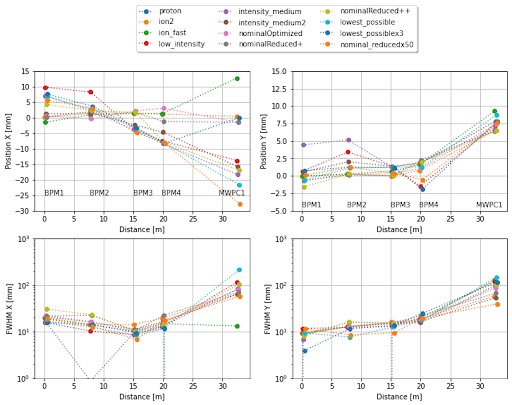
\includegraphics[width=0.95\textwidth]{images/mwpc/beam_position_evolution_MWPC.png}
    \caption{Beam position evolution along the beamline.}
    \label{fig:my_label}
\end{figure}


    \paragraph{BPMs}
    
    \paragraph{MWPC}

    The Multi Wire Proportional Chamber (MWPC) ~\cite{MWPC:CHARPAK1968262} showed promising results but could not profile the lowest intensity beams with good resolution, however the gas intensity was not optimised and the signal level could be increased in the future. 
    
    The MWPC is lcoated at the end of the beamline (behind CHARM). Its values are stored online in TIMBER (i.e. not used for fast/live monitoring). There are two MWPC, one with a signal eight times (8x) larger than the other. Each MWPC consists of two wire arrays of 32 wires, spaced at 6 mm, for each axis (horizontal and vertical). In this analysis, the values are normalized to [0, 1] and presented here as violin plots below.




\begin{figure}[H]
    \centering
    \subfigure[lower signal, horizontal position]{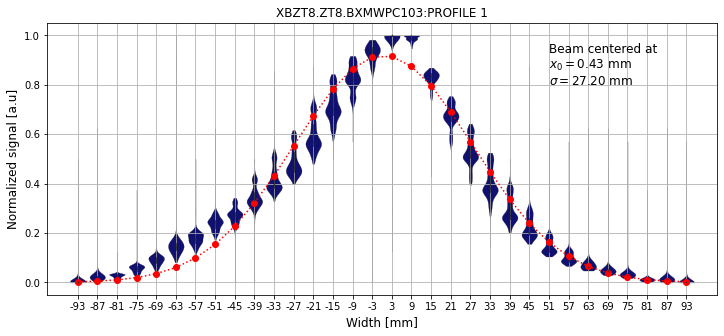
\includegraphics[width=0.49\textwidth]{images/mwpc/ion_nominal/MWPC_PROFILE_X_ion_nominal_103_1.png}} 
    \subfigure[8 x signal, horizontal position]{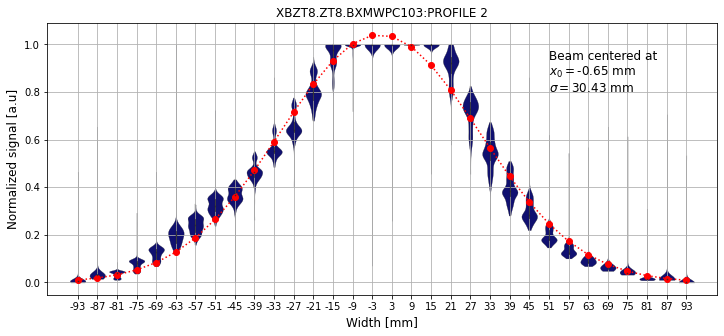
\includegraphics[width=0.49\textwidth]{images/mwpc/ion_nominal/MWPC_PROFILE_X_ion_nominal_103_2.png}} 
    \subfigure[lower signal, vertical position]{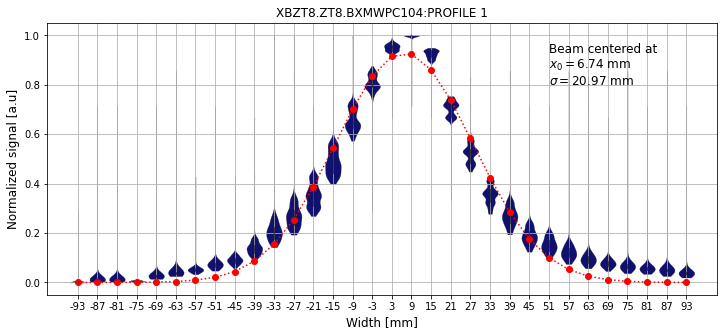
\includegraphics[width=0.49\textwidth]{images/mwpc/ion_nominal/MWPC_PROFILE_X_ion_nominal_104_1.png}}
    \subfigure[8 x signal, vertical position]{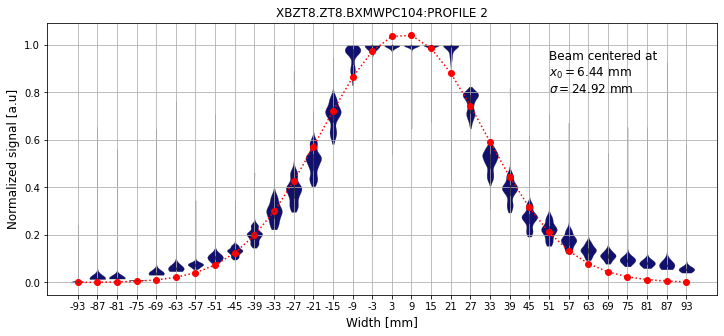
\includegraphics[width=0.49\textwidth]{images/mwpc/ion_nominal/MWPC_PROFILE_X_ion_nominal_104_2.png}}
    \caption{MWPC profile, nominal ion operation}
    \label{fig:mwpc-ion-nominal}
\end{figure}
    


\begin{figure}[H]
    \centering
    \subfigure[lower signal, horizontal position]{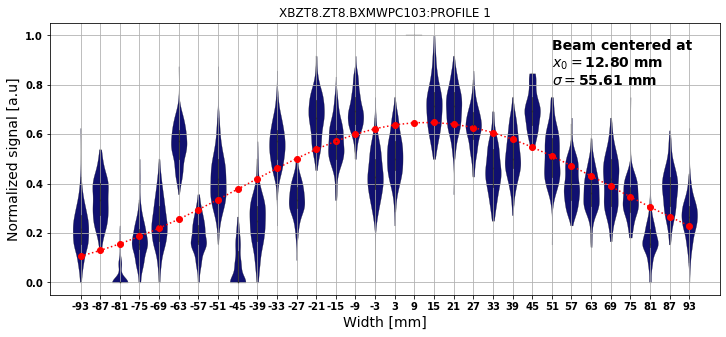
\includegraphics[width=0.49\textwidth]{images/mwpc/fast_extraction/MWPC_PROFILE_X_fast_extraction_103_1.png}} 
    \subfigure[8 x signal, horizontal position]{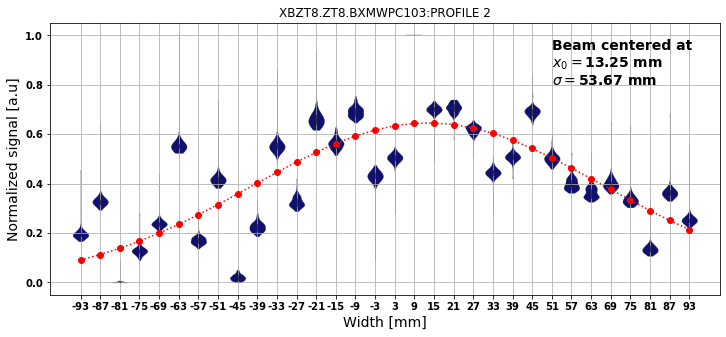
\includegraphics[width=0.49\textwidth]{images/mwpc/fast_extraction/MWPC_PROFILE_X_fast_extraction_103_2.png}} 
    \subfigure[lower signal, vertical position]{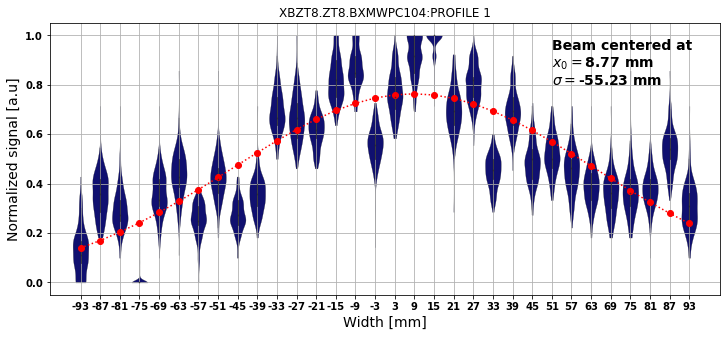
\includegraphics[width=0.49\textwidth]{images/mwpc/fast_extraction/MWPC_PROFILE_X_fast_extraction_104_1.png}}
    \subfigure[8 x signal, vertical position]{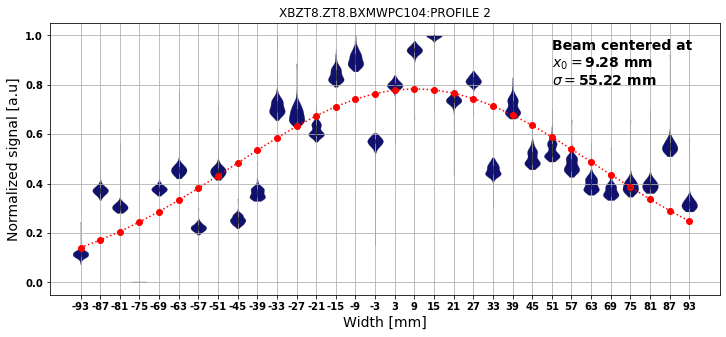
\includegraphics[width=0.49\textwidth]{images/mwpc/fast_extraction/MWPC_PROFILE_X_fast_extraction_104_2.png}}
    \caption{MWPC profile, fast extraction}
    \label{fig:mwpc-fast-extraction}
\end{figure}
    

\begin{figure}[H]
    \centering
    \subfigure[lower signal, horizontal position]{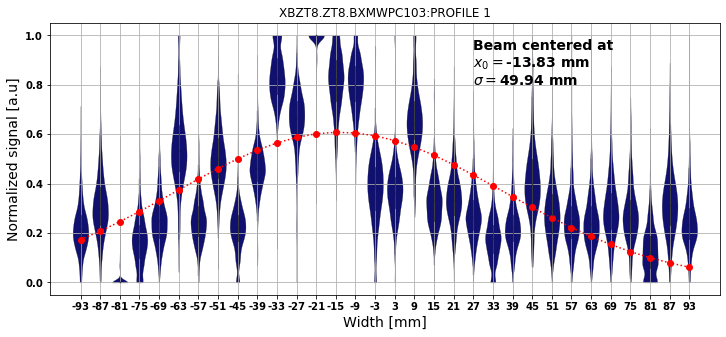
\includegraphics[width=0.49\textwidth]{images/mwpc/lowest_intensity/MWPC_PROFILE_X_low_intensity_103_1.png}} 
    \subfigure[8 x signal, horizontal position]{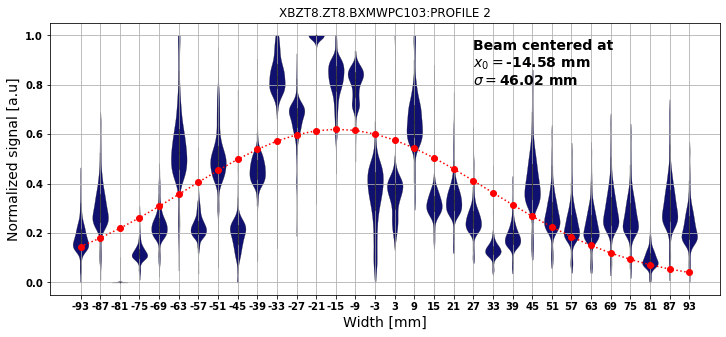
\includegraphics[width=0.49\textwidth]{images/mwpc/lowest_intensity/MWPC_PROFILE_X_low_intensity_103_2.png}} 
    \subfigure[lower signal, vertical position]{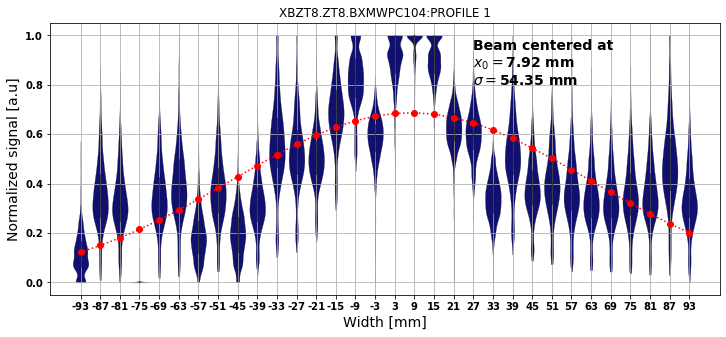
\includegraphics[width=0.49\textwidth]{images/mwpc/lowest_intensity/MWPC_PROFILE_X_low_intensity_104_1.png}}
    \subfigure[8 x signal, vertical position]{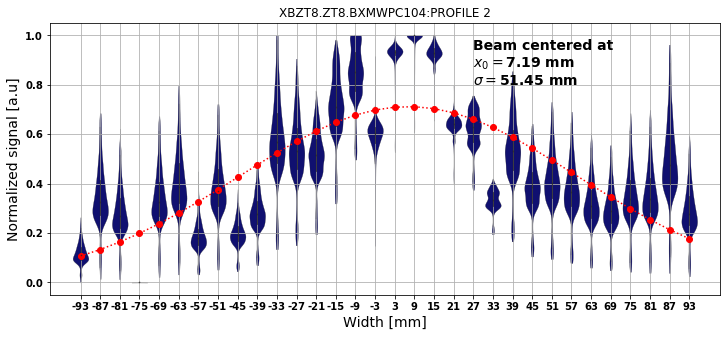
\includegraphics[width=0.49\textwidth]{images/mwpc/lowest_intensity/MWPC_PROFILE_X_low_intensity_104_2.png}}
    \caption{MWPC profile, low intensity operation}
    \label{fig:mwpc-low-intensity}
\end{figure}
    
    
\begin{figure}[H]
    \centering
    \subfigure[lower signal, horizontal position]{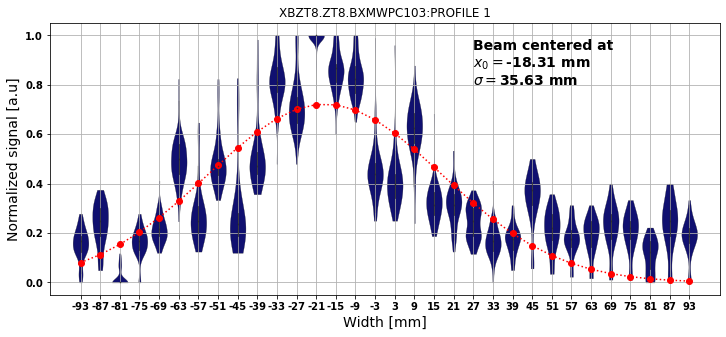
\includegraphics[width=0.49\textwidth]{images/mwpc/intensity_medium/MWPC_PROFILE_X_intensity_medium_103_1.png}} 
    \subfigure[8 x signal, horizontal position]{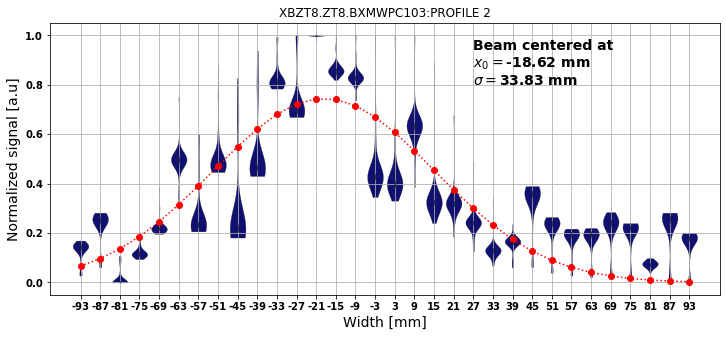
\includegraphics[width=0.49\textwidth]{images/mwpc/intensity_medium/MWPC_PROFILE_X_intensity_medium_103_2.png}} 
    \subfigure[lower signal, vertical position]{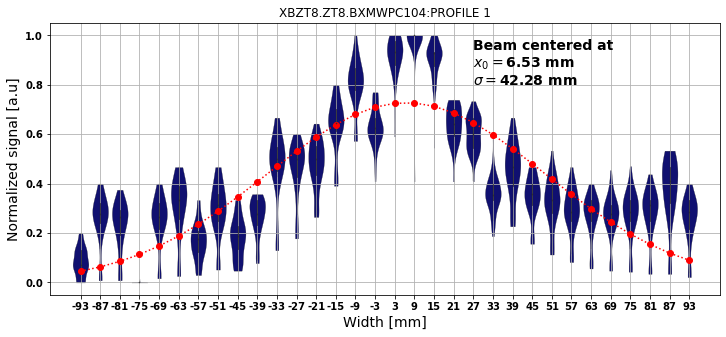
\includegraphics[width=0.49\textwidth]{images/mwpc/intensity_medium/MWPC_PROFILE_X_intensity_medium_104_1.png}}
    \subfigure[8 x signal, vertical position]{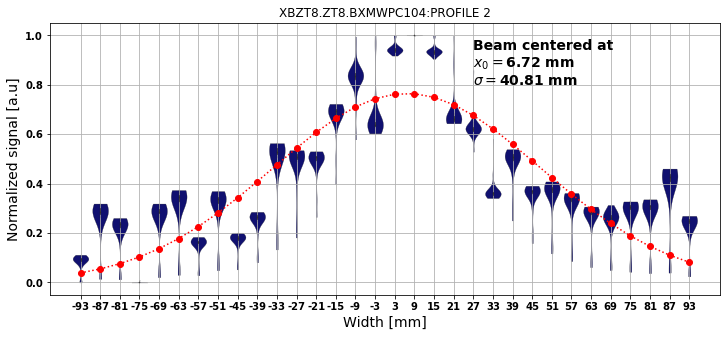
\includegraphics[width=0.49\textwidth]{images/mwpc/intensity_medium/MWPC_PROFILE_X_intensity_medium_104_2.png}}
    \caption{MWPC profile, medium intensity operation}
    \label{fig:mwpc-medium-intensity}
\end{figure}
    
    
\begin{figure}[H]
    \centering
    \subfigure[lower signal, horizontal position]{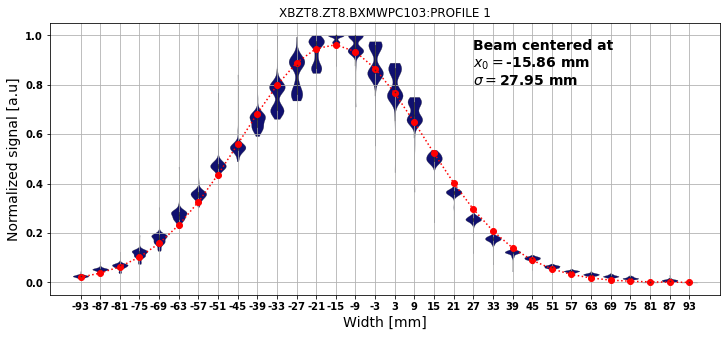
\includegraphics[width=0.49\textwidth]{images/mwpc/intensity_medium_high/MWPC_PROFILE_X_intensity_medium_high_103_1.png}} 
    \subfigure[8 x signal, horizontal position]{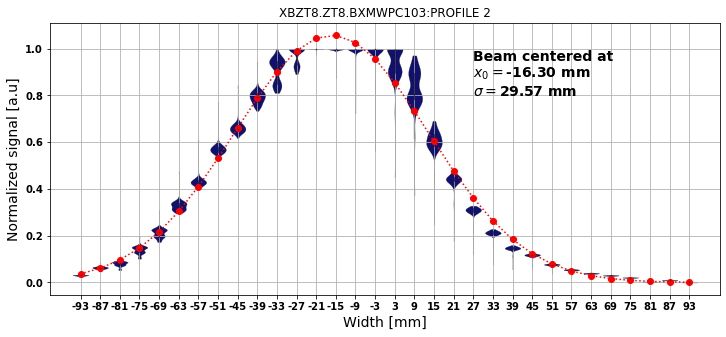
\includegraphics[width=0.49\textwidth]{images/mwpc/intensity_medium_high/MWPC_PROFILE_X_intensity_medium_high_103_2.png}} 
    \subfigure[lower signal, vertical position]{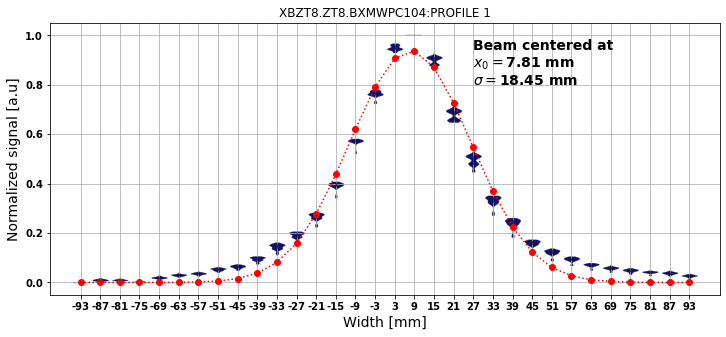
\includegraphics[width=0.49\textwidth]{images/mwpc/intensity_medium_high/MWPC_PROFILE_X_intensity_medium_high_104_1.png}}
    \subfigure[8 x signal, vertical position]{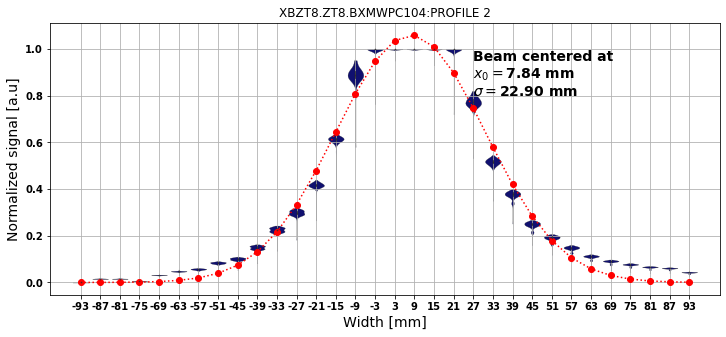
\includegraphics[width=0.49\textwidth]{images/mwpc/intensity_medium_high/MWPC_PROFILE_X_intensity_medium_high_104_2.png}}
    \caption{MWPC profile, medium high intensity operation}
    \label{fig:mwpc-medium-high-intensity}
\end{figure}
    
    
\begin{figure}[H]
    \centering
    \subfigure[lower signal, horizontal position]{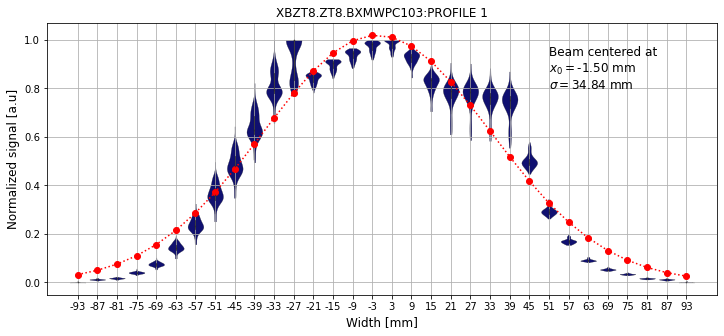
\includegraphics[width=0.49\textwidth]{images/mwpc/nominalOptimized/MWPC_PROFILE_X_ion_nominalOptimized_103_1.png}} 
    \subfigure[8 x signal, horizontal position]{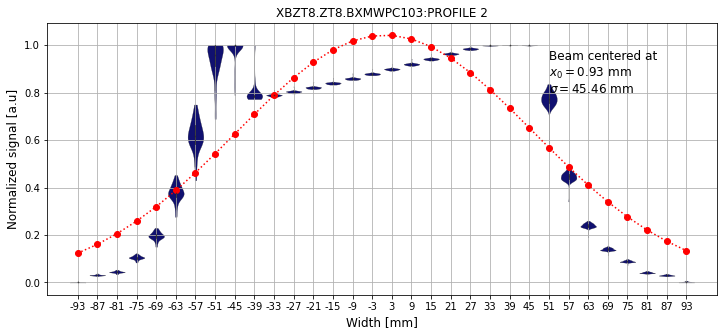
\includegraphics[width=0.49\textwidth]{images/mwpc/nominalOptimized/MWPC_PROFILE_X_ion_nominalOptimized_103_2.png}} 
    \subfigure[lower signal, vertical position]{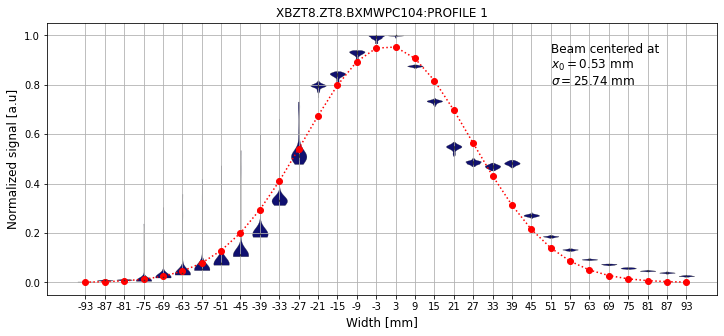
\includegraphics[width=0.49\textwidth]{images/mwpc/nominalOptimized/MWPC_PROFILE_X_ion_nominalOptimized_104_1.png}}
    \subfigure[8 x signal, vertical position]{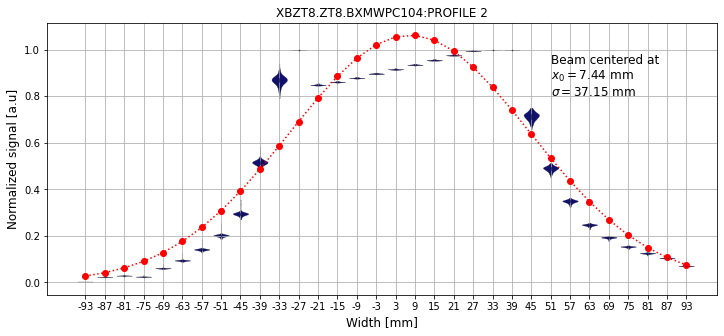
\includegraphics[width=0.49\textwidth]{images/mwpc/nominalOptimized/MWPC_PROFILE_X_ion_nominalOptimized_104_2.png}}
    \caption{MWPC profile, nominal optimized operation}
    \label{fig:mwpc-nominal-optimized-intensity}
\end{figure}

    
\begin{figure}[H]
    \centering
    \subfigure[lower signal, horizontal position]{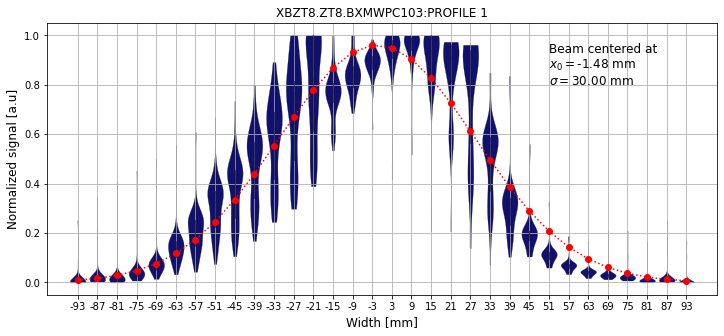
\includegraphics[width=0.49\textwidth]{images/mwpc/nominalReduced+/MWPC_PROFILE_X_ion_nominalReduced+_103_1.png}} 
    \subfigure[8 x signal, horizontal position]{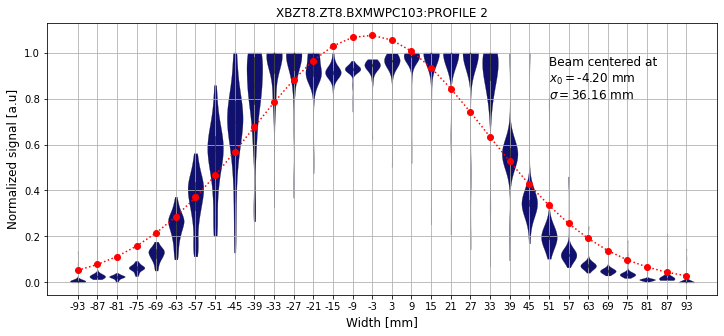
\includegraphics[width=0.49\textwidth]{images/mwpc/nominalReduced+/MWPC_PROFILE_X_ion_nominalReduced+_103_2.png}} 
    \subfigure[lower signal, vertical position]{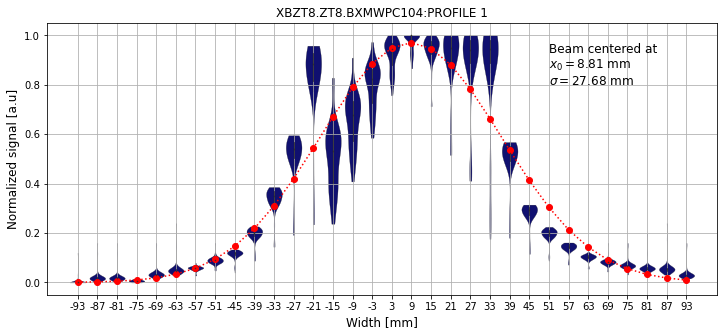
\includegraphics[width=0.49\textwidth]{images/mwpc/nominalReduced+/MWPC_PROFILE_X_ion_nominalReduced+_104_1.png}}
    \subfigure[8 x signal, vertical position]{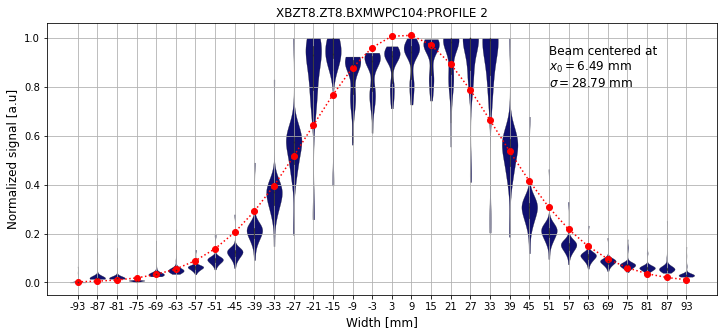
\includegraphics[width=0.49\textwidth]{images/mwpc/nominalReduced+/MWPC_PROFILE_X_ion_nominalReduced+_104_2.png}}
    \caption{MWPC profile, nominal reduced+ operation}
    \label{fig:mwpc-nominal-reduced+-intensity}
\end{figure}
   
  
    
\begin{figure}[H]
    \centering
    \subfigure[lower signal, horizontal position]{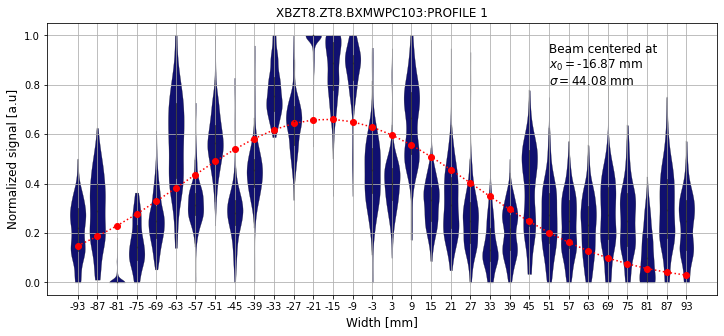
\includegraphics[width=0.49\textwidth]{images/mwpc/nominalReduced++/MWPC_PROFILE_X_ion_nominalReduced++_103_1.png}} 
    \subfigure[8 x signal, horizontal position]{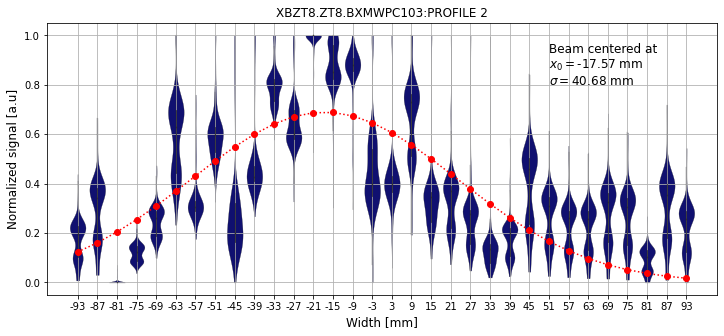
\includegraphics[width=0.49\textwidth]{images/mwpc/nominalReduced++/MWPC_PROFILE_X_ion_nominalReduced++_103_2.png}} 
    \subfigure[lower signal, vertical position]{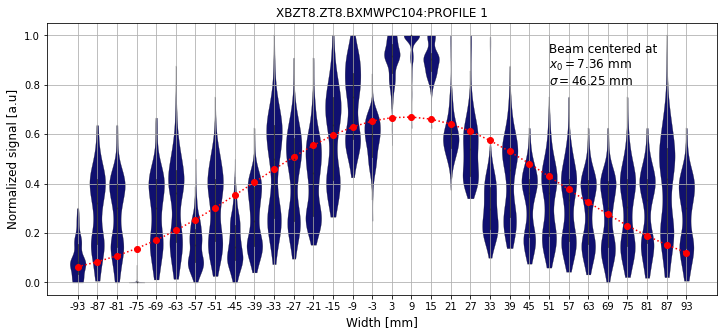
\includegraphics[width=0.49\textwidth]{images/mwpc/nominalReduced++/MWPC_PROFILE_X_ion_nominalReduced++_104_1.png}}
    \subfigure[8 x signal, vertical position]{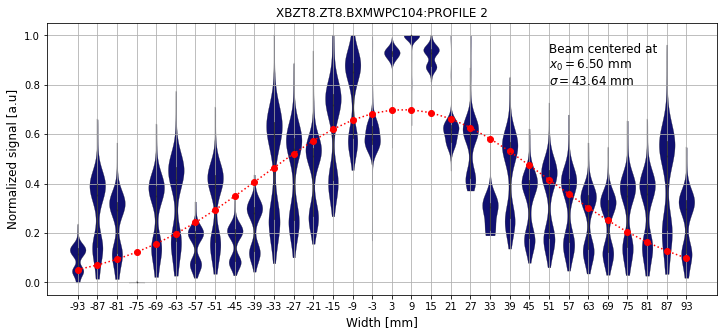
\includegraphics[width=0.49\textwidth]{images/mwpc/nominalReduced++/MWPC_PROFILE_X_ion_nominalReduced++_104_2.png}}
    \caption{MWPC profile, nominal reduced++ operation}
    \label{fig:mwpc-nominal-reduced++-intensity}
\end{figure}
    
  
 
 \begin{figure}[H]
    \centering
    \subfigure[lower signal, horizontal position]{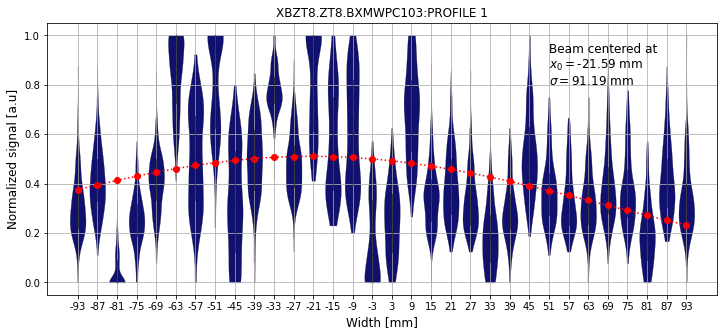
\includegraphics[width=0.49\textwidth]{images/mwpc/lowest_possible/MWPC_PROFILE_X_ion_lowest_possible_103_1.png}} 
    \subfigure[8 x signal, horizontal position]{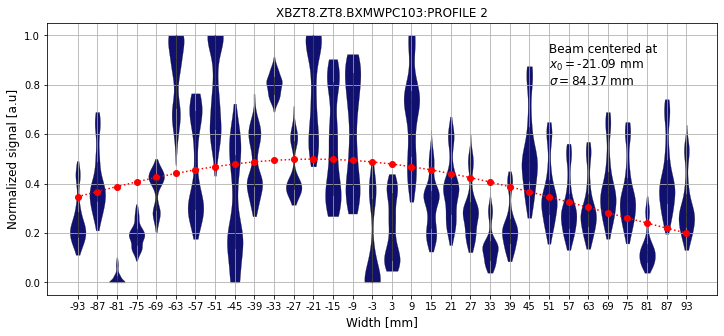
\includegraphics[width=0.49\textwidth]{images/mwpc/lowest_possible/MWPC_PROFILE_X_ion_lowest_possible_103_2.png}} 
    \subfigure[lower signal, vertical position]{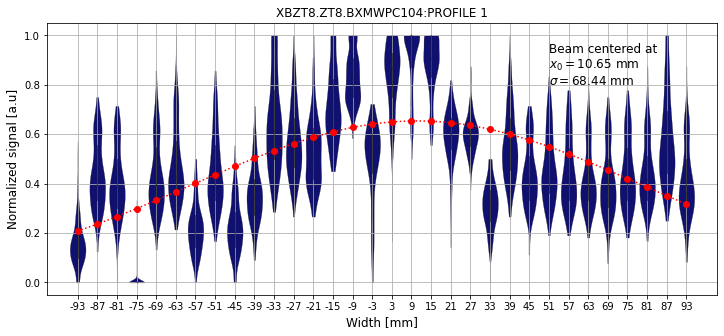
\includegraphics[width=0.49\textwidth]{images/mwpc/lowest_possible/MWPC_PROFILE_X_ion_lowest_possible_104_1.png}}
    \subfigure[8 x signal, vertical position]{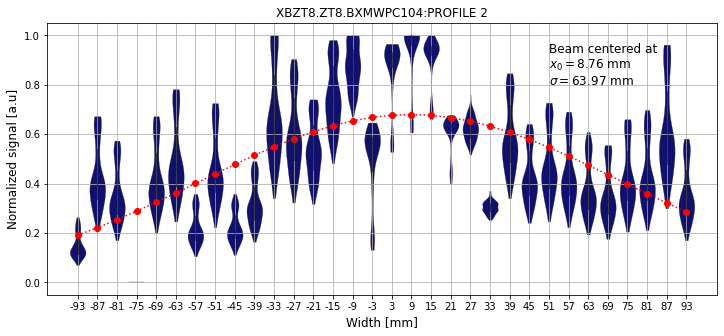
\includegraphics[width=0.49\textwidth]{images/mwpc/lowest_possible/MWPC_PROFILE_X_ion_lowest_possible_104_2.png}}
    \caption{MWPC profile, lowest possible operation}
    \label{fig:mwpc-lowest-possible-intensity}
\end{figure}
    
 
 
 
 \begin{figure}[H]
    \centering
    \subfigure[lower signal, horizontal position]{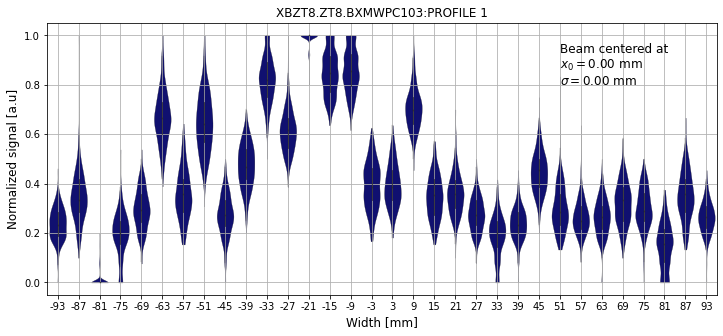
\includegraphics[width=0.49\textwidth]{images/mwpc/lowest_possiblex3/MWPC_PROFILE_X_ion_lowest_possible_x3_103_1.png}} 
    \subfigure[8 x signal, horizontal position]{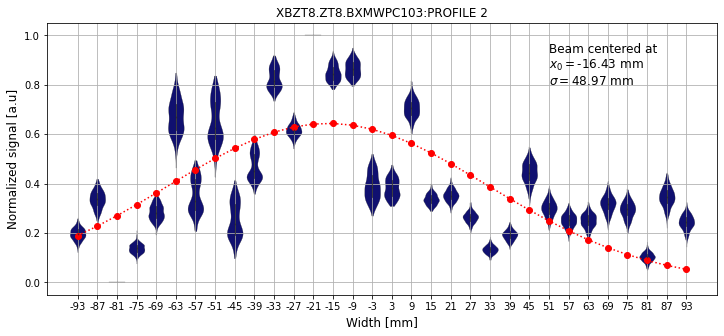
\includegraphics[width=0.49\textwidth]{images/mwpc/lowest_possiblex3/MWPC_PROFILE_X_ion_lowest_possible_x3_103_2.png}} 
    \subfigure[lower signal, vertical position]{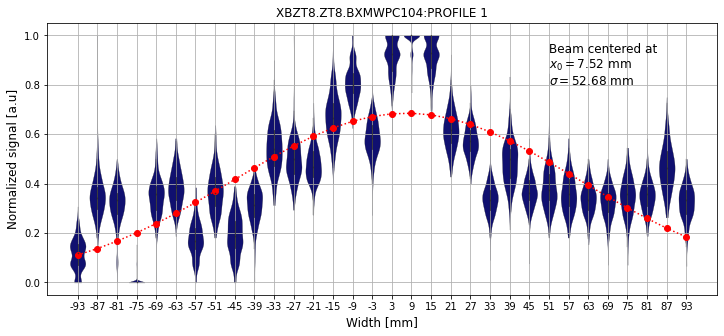
\includegraphics[width=0.49\textwidth]{images/mwpc/lowest_possiblex3/MWPC_PROFILE_X_ion_lowest_possible_x3_104_1.png}}
    \subfigure[8 x signal, vertical position]{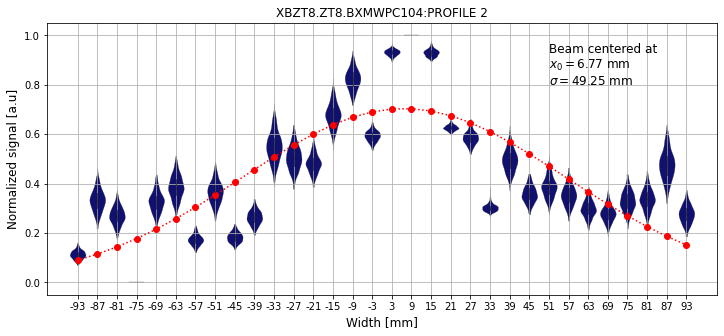
\includegraphics[width=0.49\textwidth]{images/mwpc/lowest_possiblex3/MWPC_PROFILE_X_ion_lowest_possible_x3_104_2.png}}
    \caption{MWPC profile, lowest possible x3 operation}
    \label{fig:mwpc-lowest-possiblex3-intensity}
\end{figure}

 \begin{figure}[H]
    \centering
    \subfigure[lower signal, horizontal position]{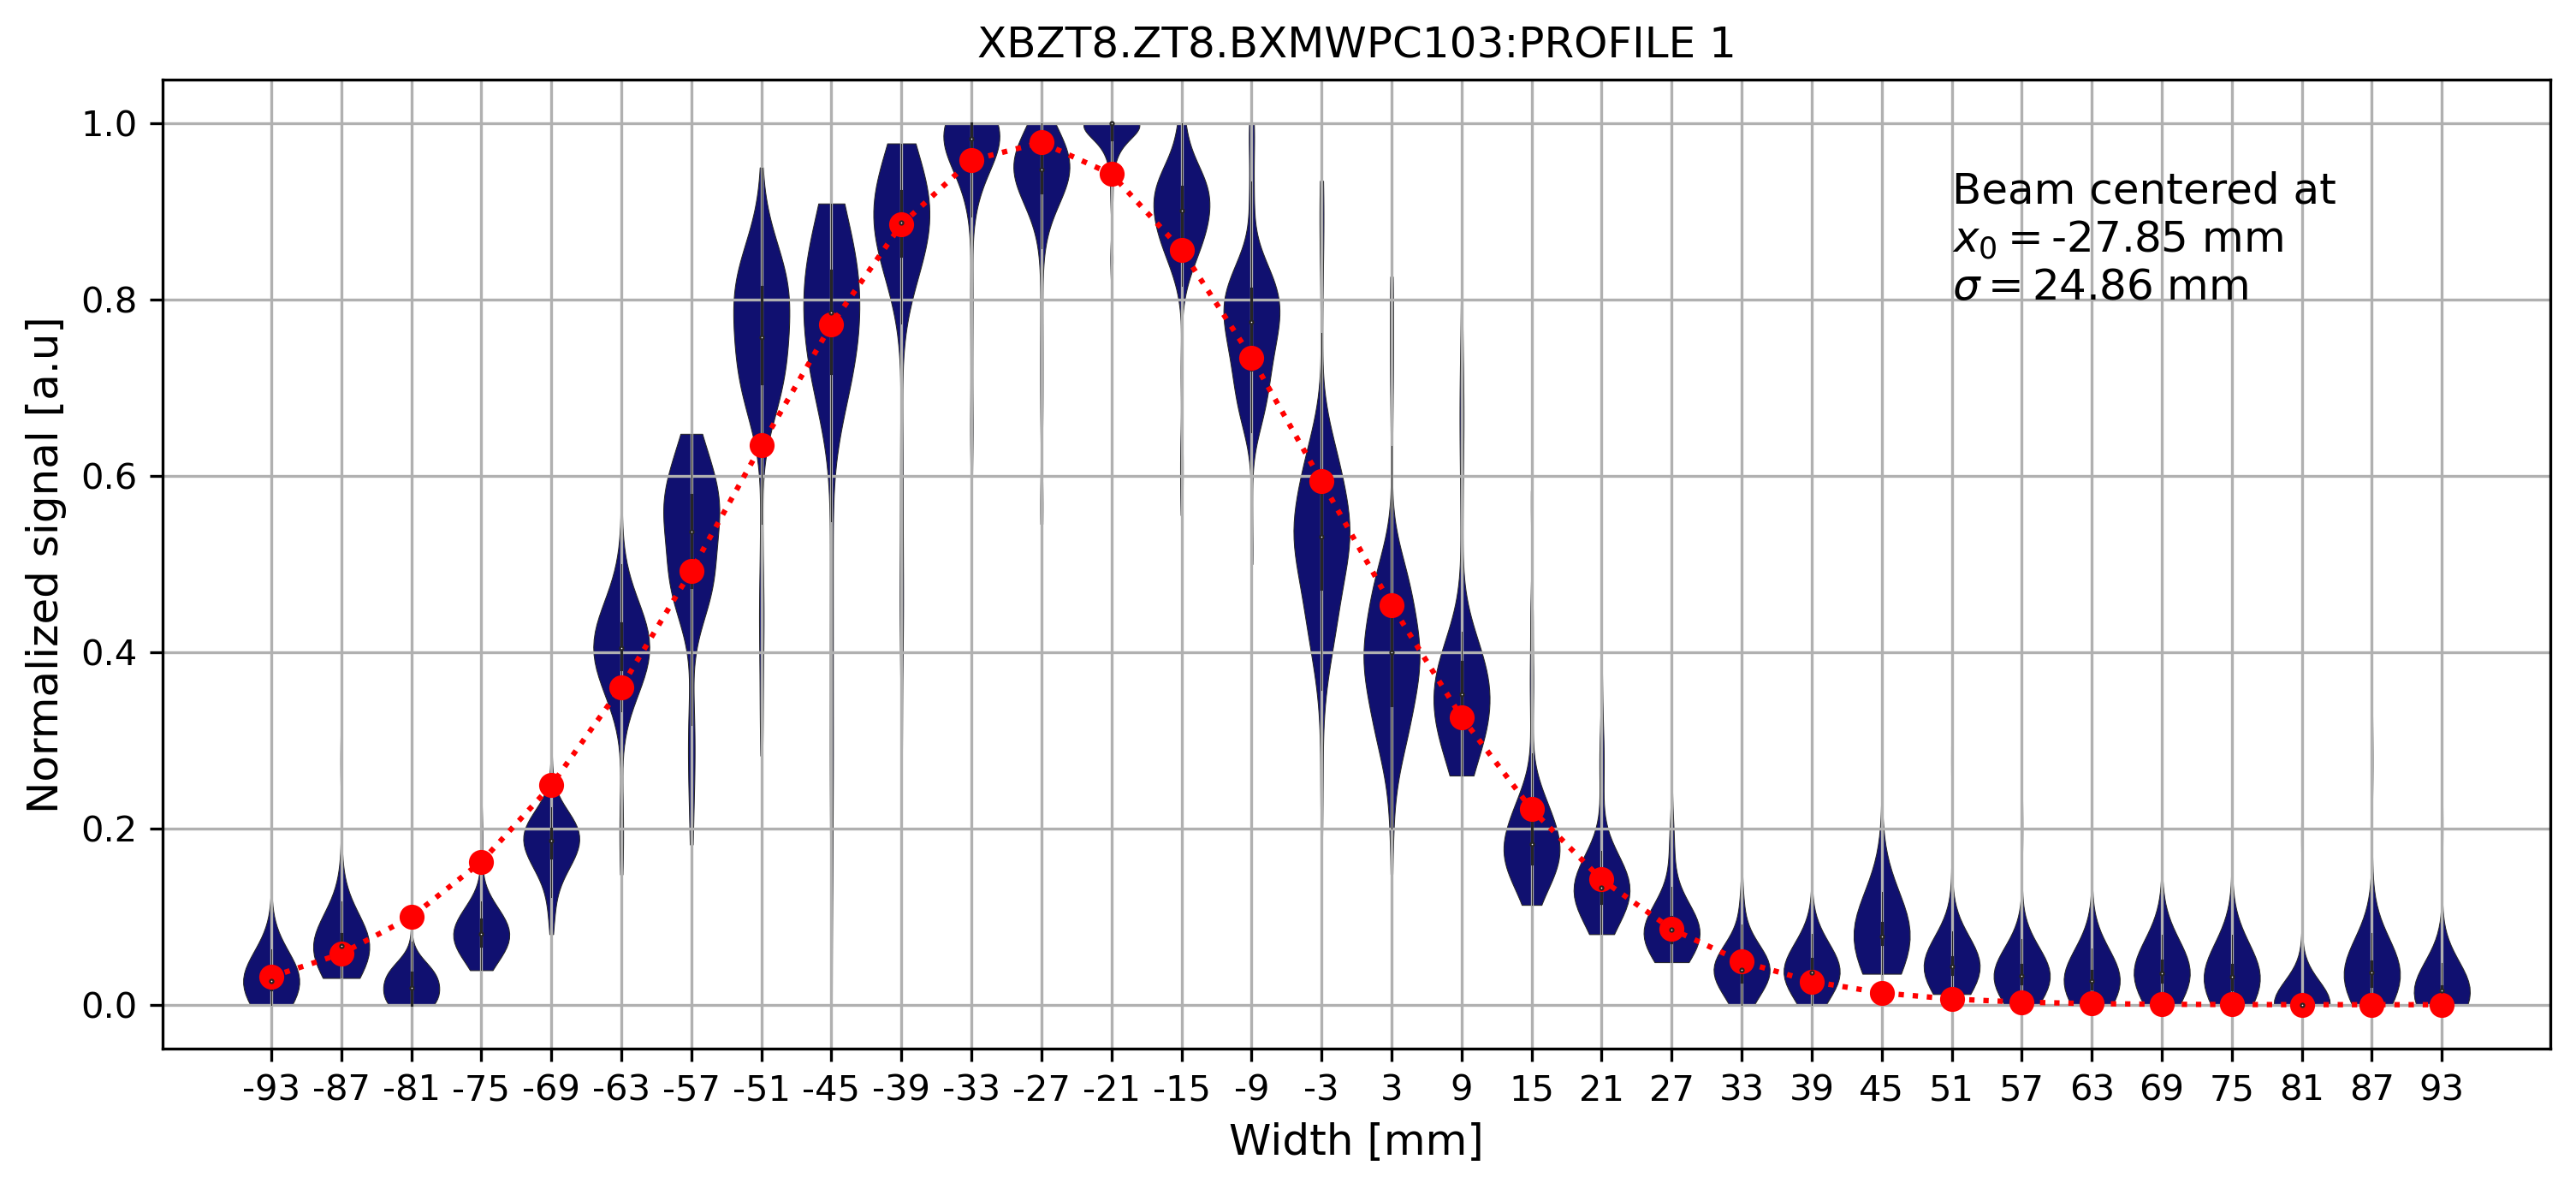
\includegraphics[width=0.49\textwidth]{images/mwpc/nominal_reduced_x50/MWPC_PROFILE_X_ion_nominal_reduced_x50_103_1.png}} 
    \subfigure[8 x signal, horizontal position]{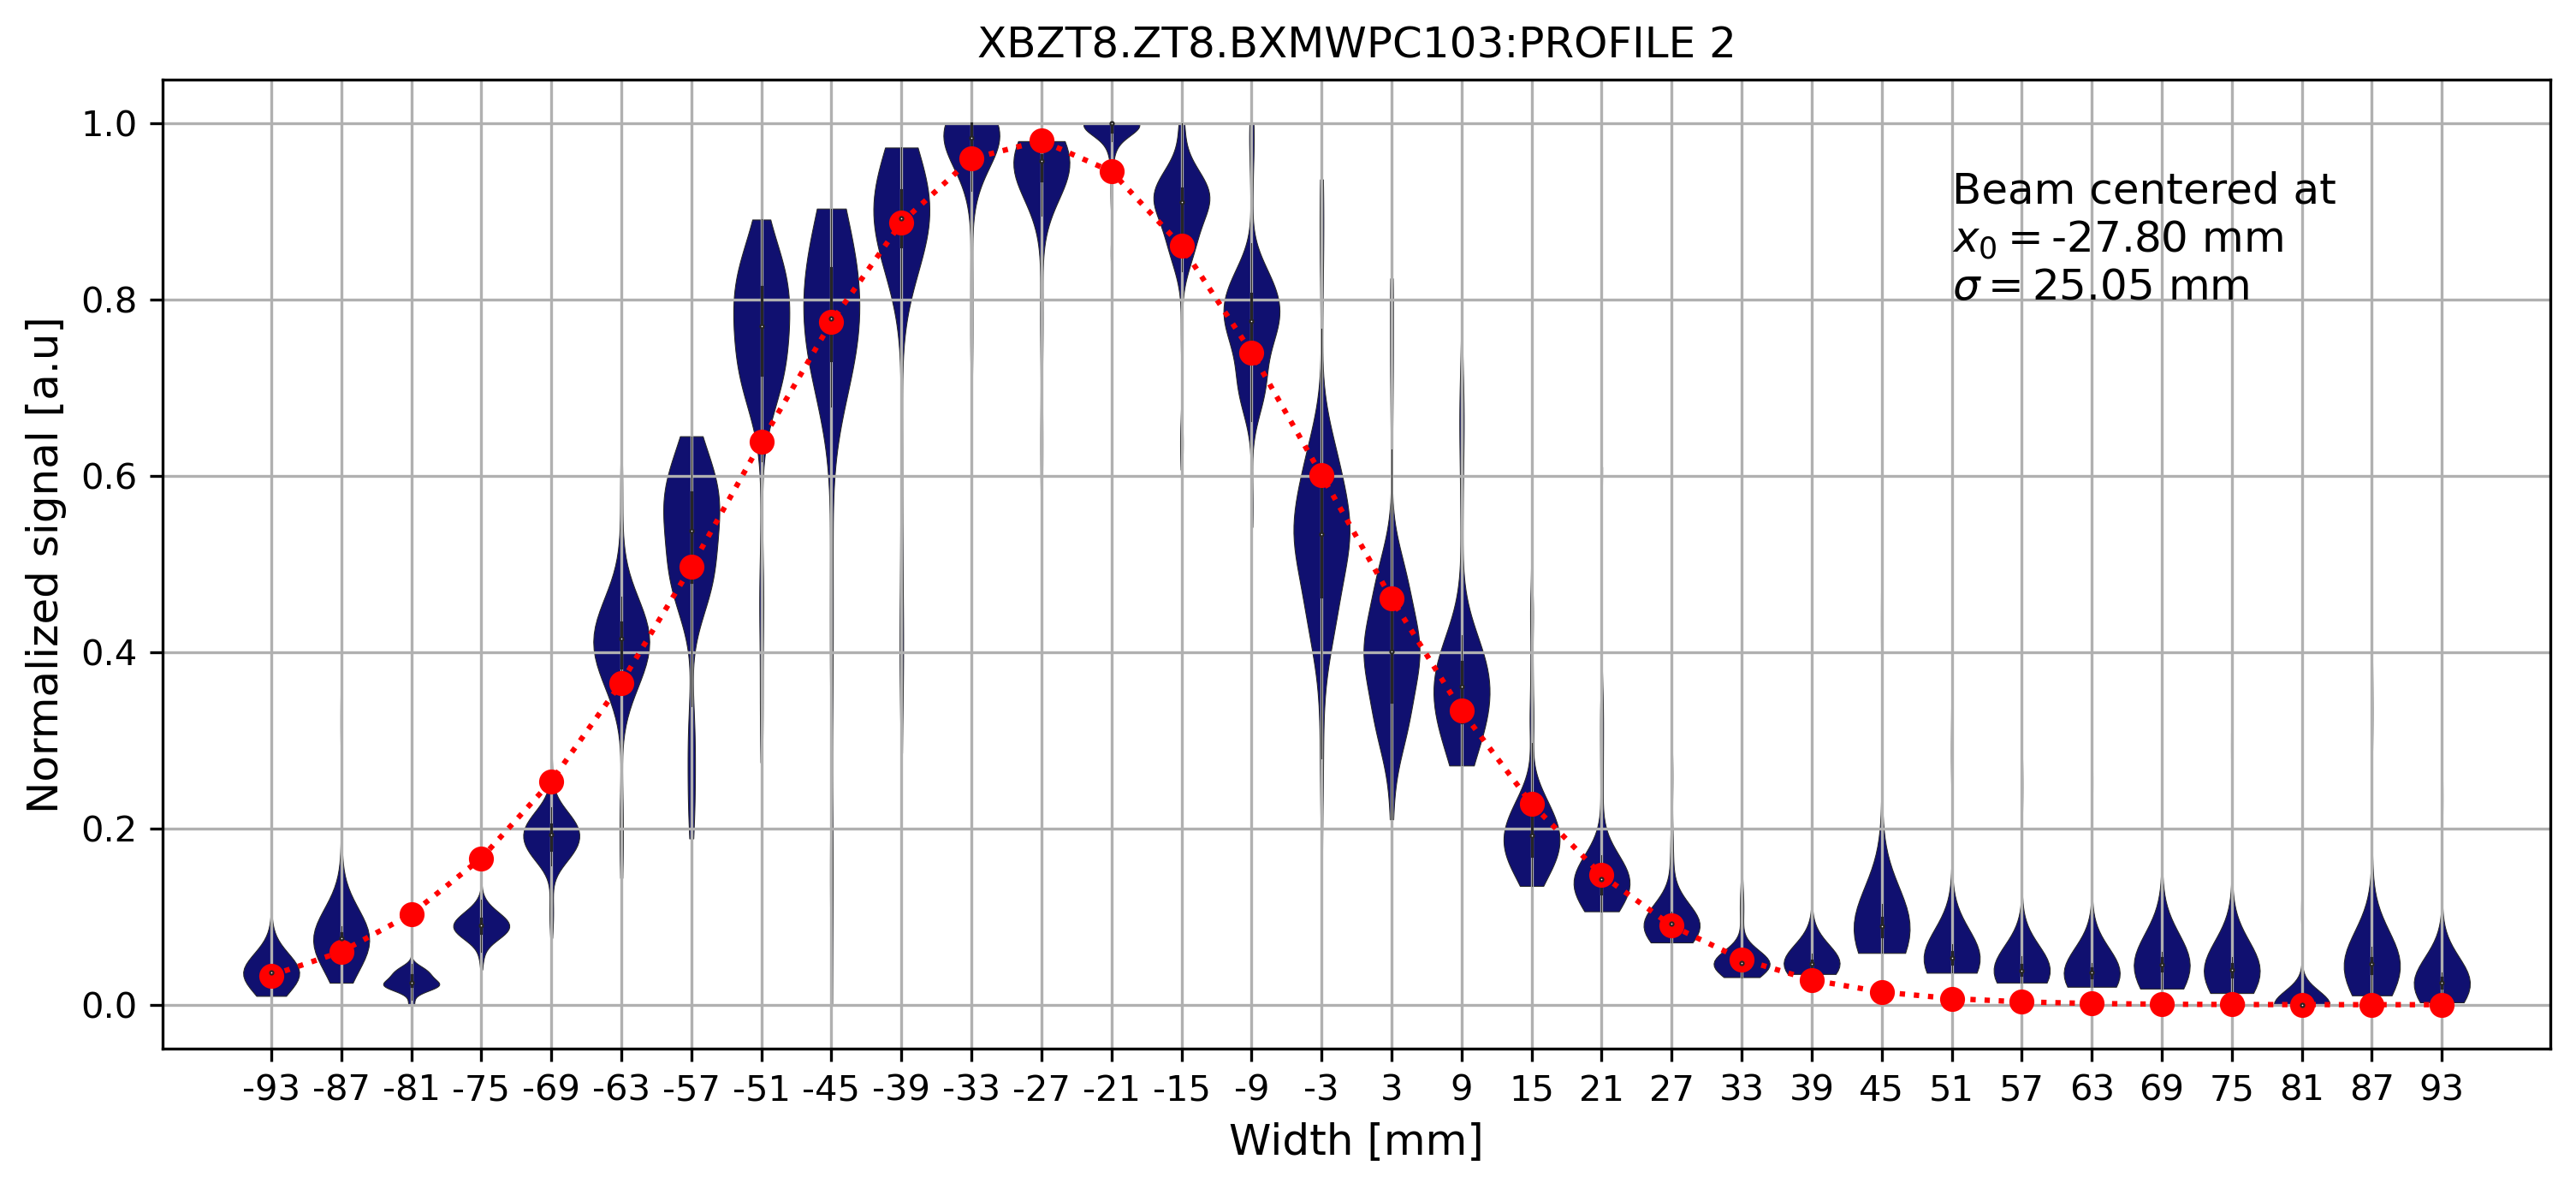
\includegraphics[width=0.49\textwidth]{images/mwpc/nominal_reduced_x50/MWPC_PROFILE_X_ion_nominal_reduced_x50_103_2.png}} 
    \subfigure[lower signal, vertical position]{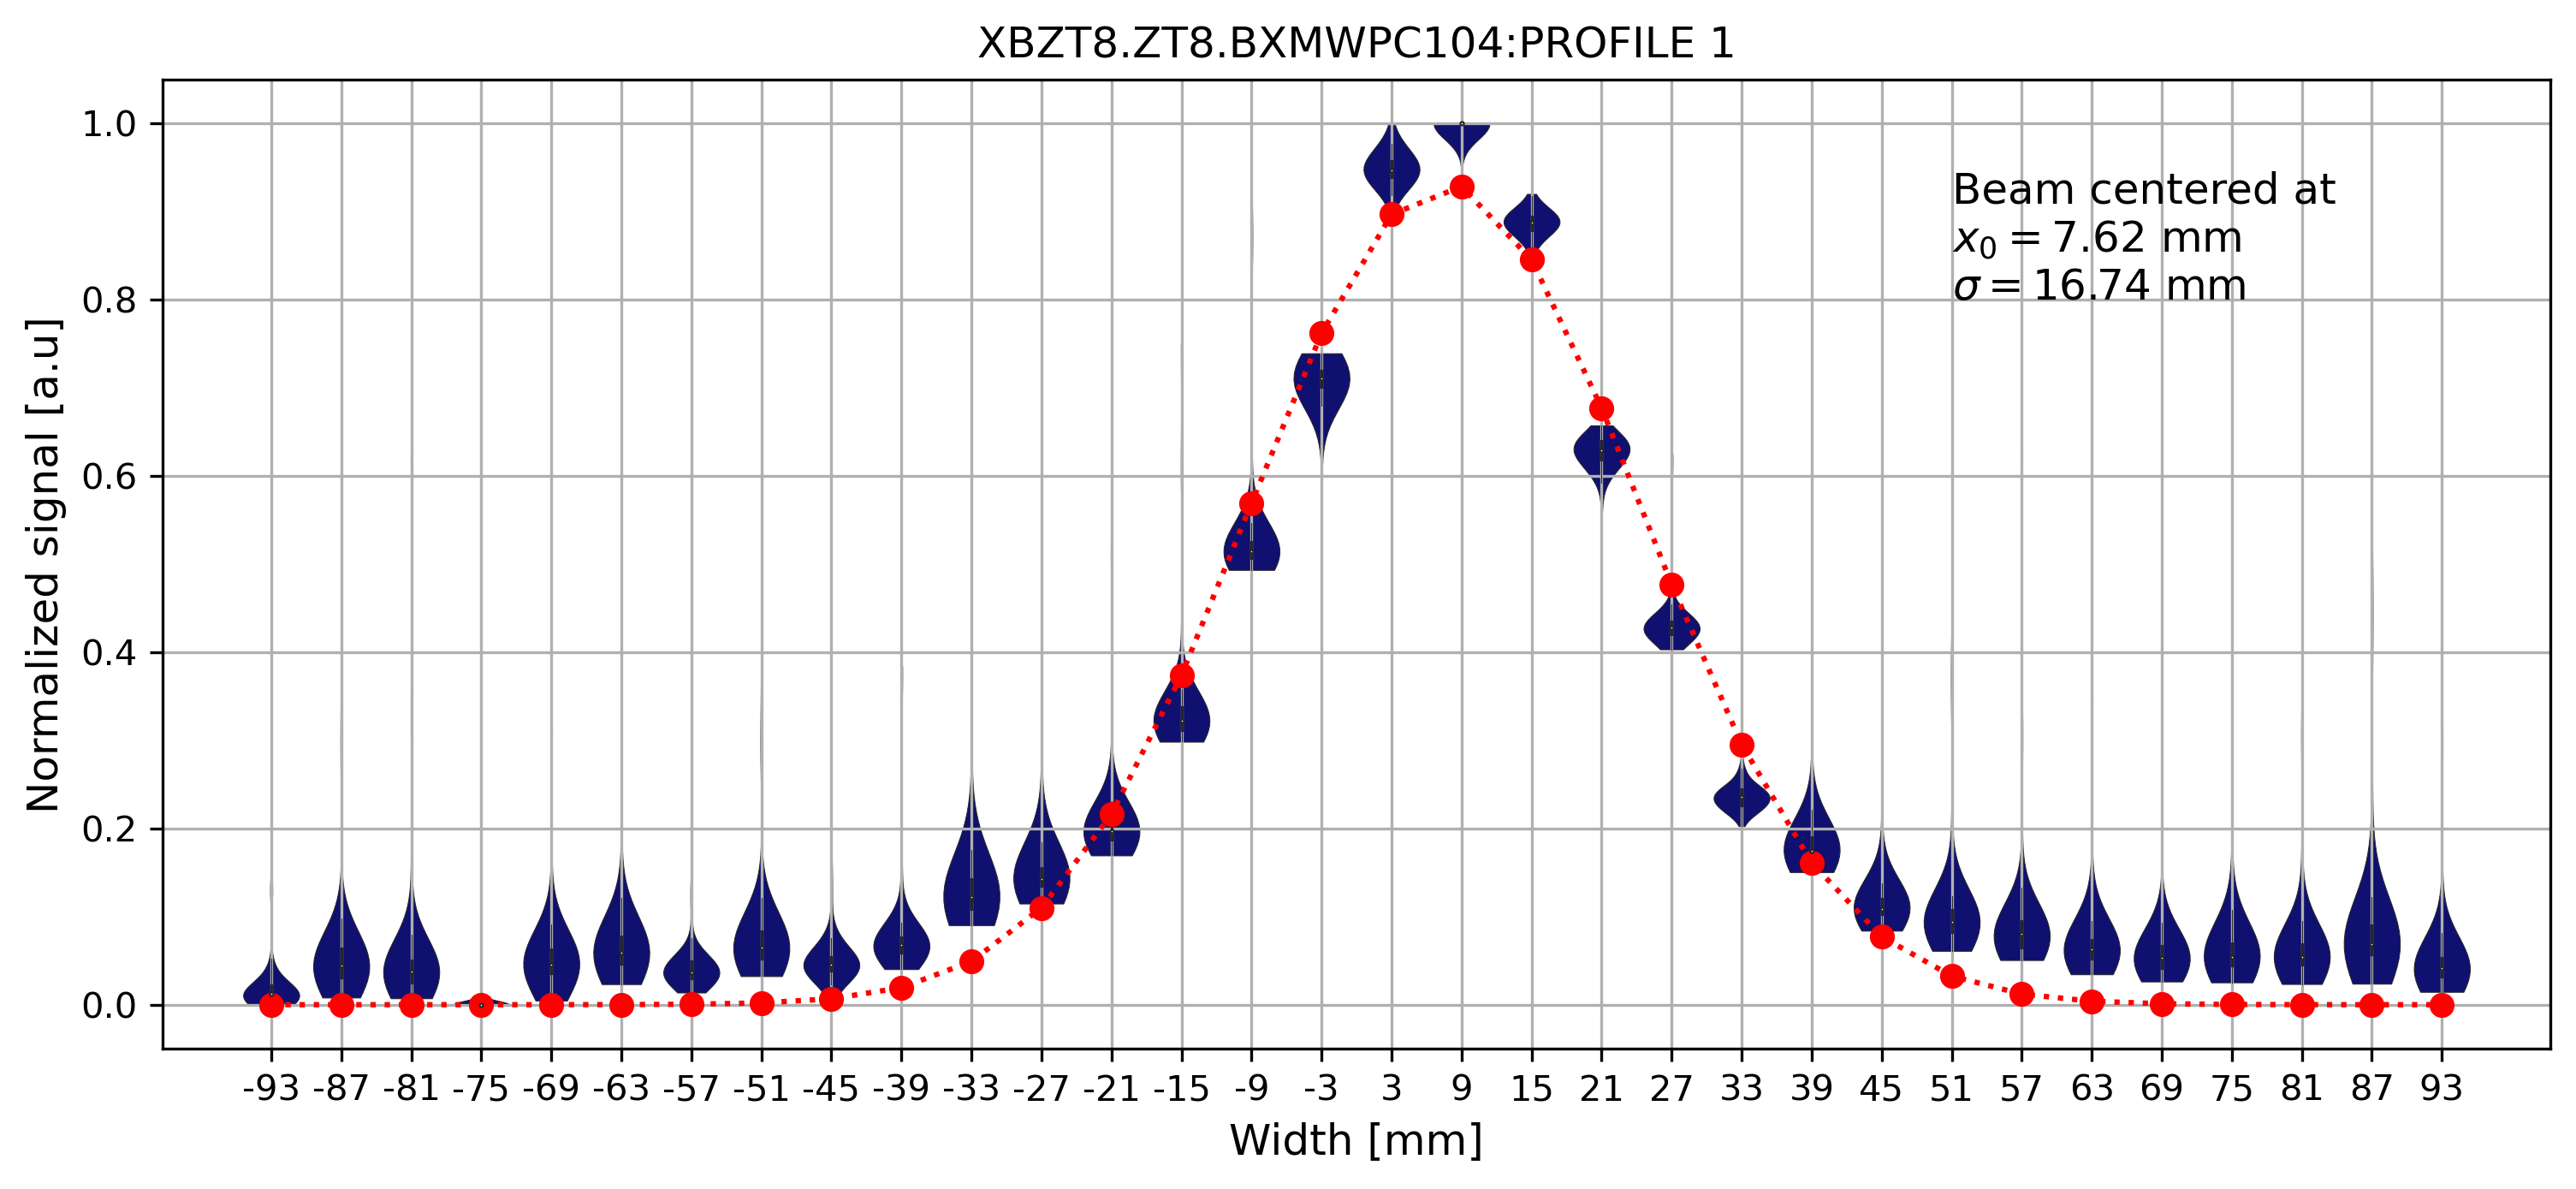
\includegraphics[width=0.49\textwidth]{images/mwpc/nominal_reduced_x50/MWPC_PROFILE_X_ion_nominal_reduced_x50_104_1.png}}
    \subfigure[8 x signal, vertical position]{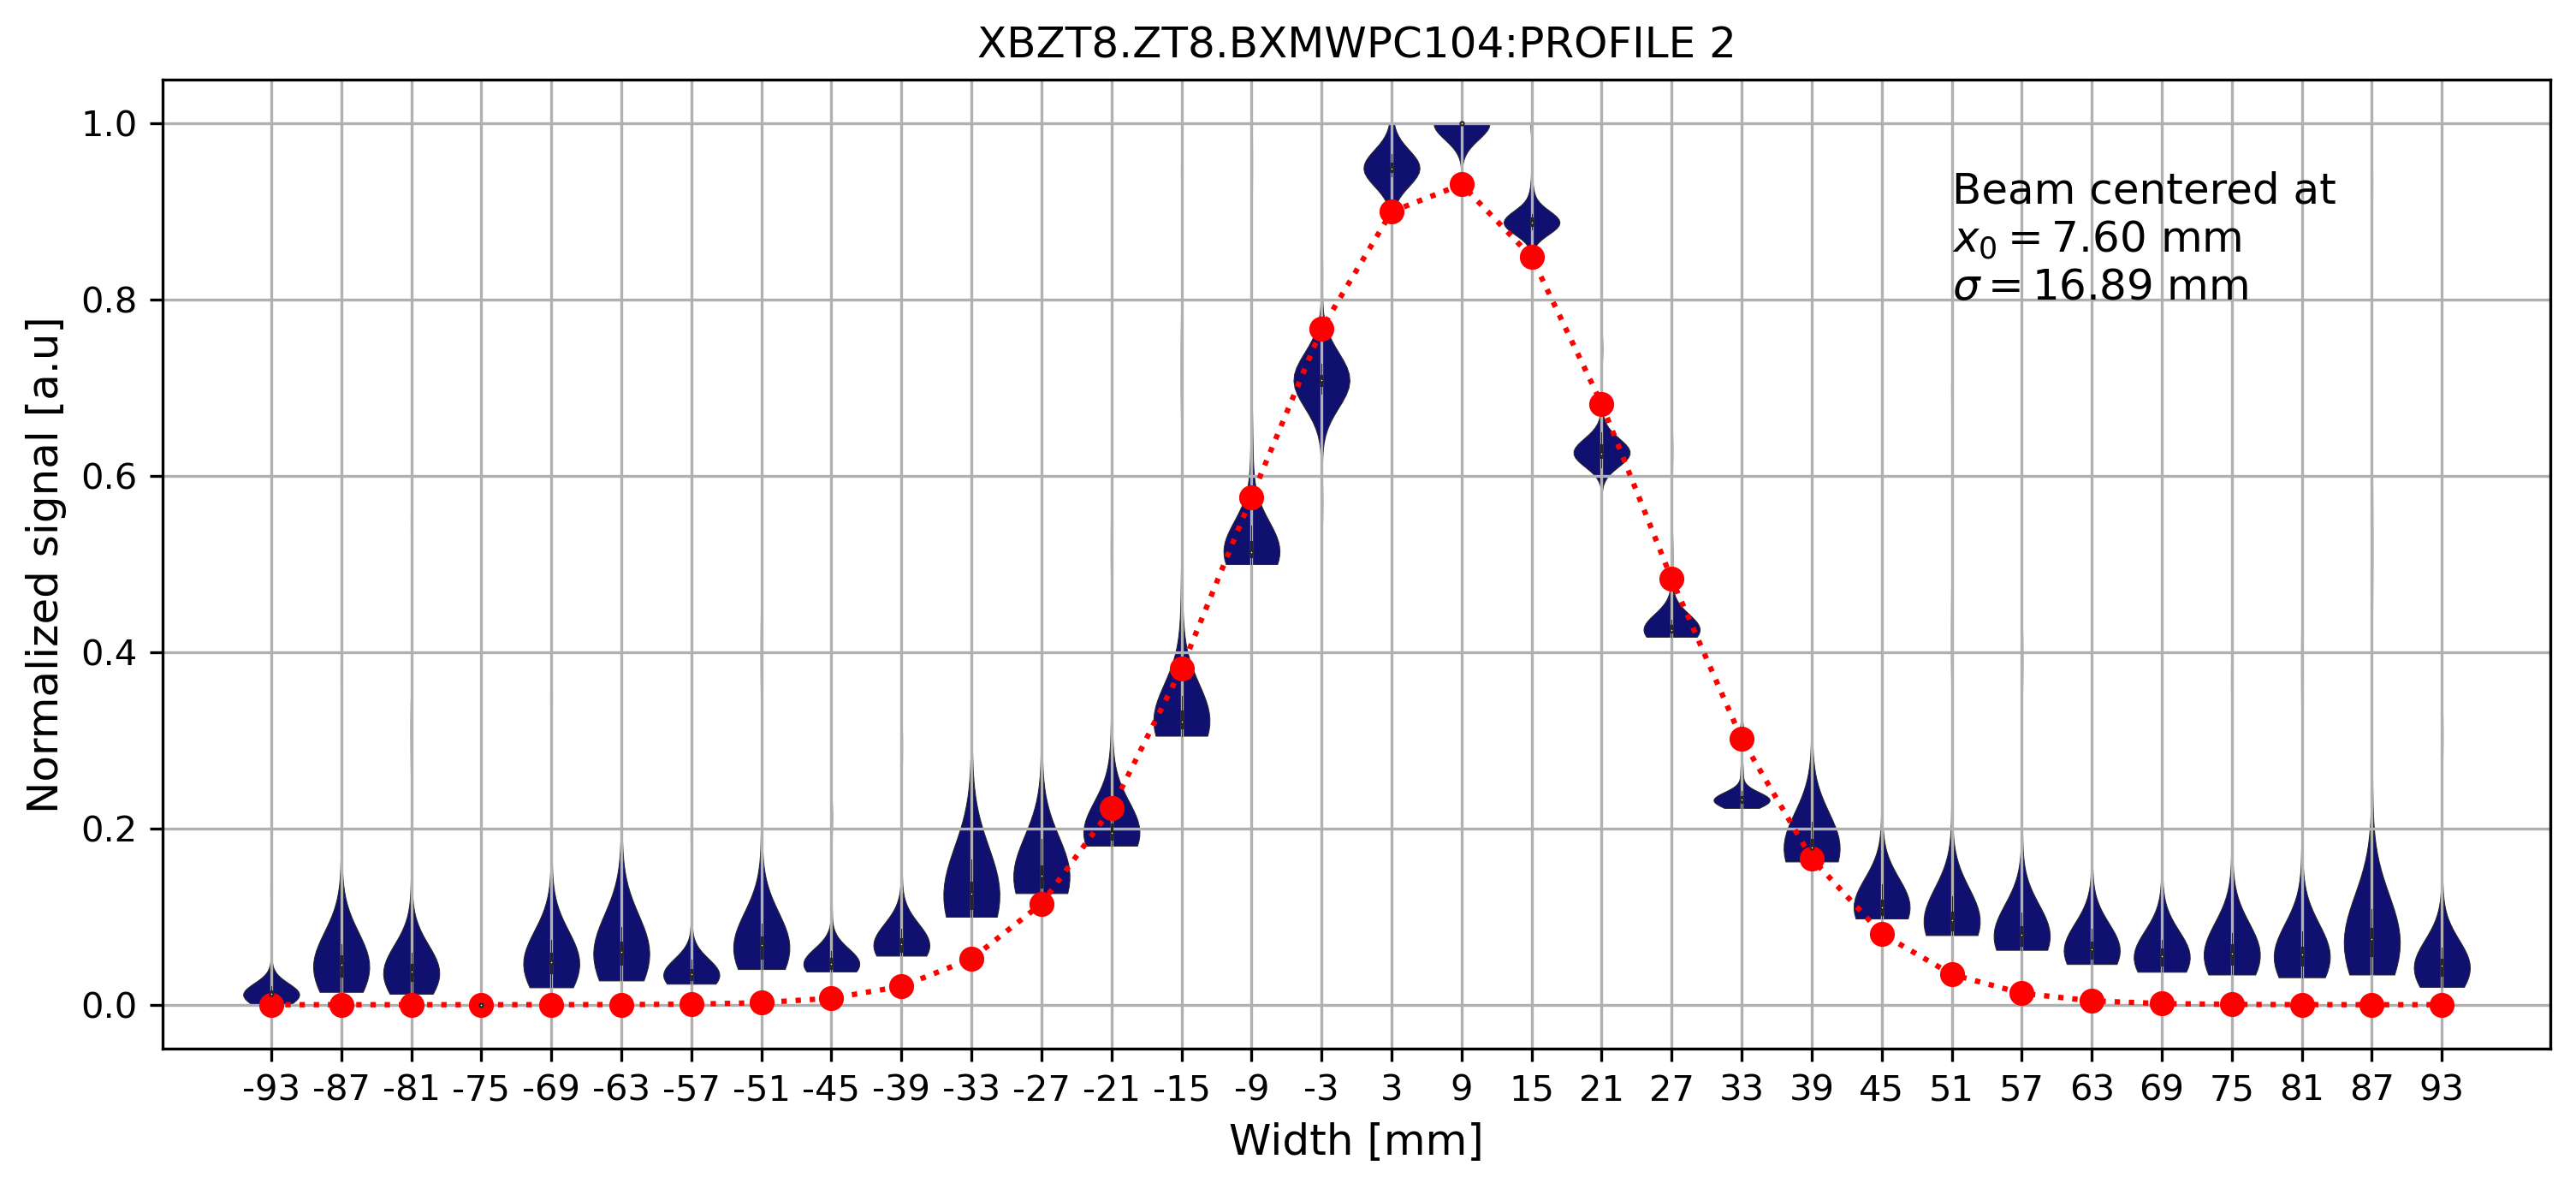
\includegraphics[width=0.49\textwidth]{images/mwpc/nominal_reduced_x50/MWPC_PROFILE_X_ion_nominal_reduced_x50_104_2.png}}
    \caption{MWPC profile, nominal reduced x50 operation}
    \label{fig:mwpc-nominal-reduced-x50-intensity}
\end{figure}
    
        
        % Kacper, Natalia
        \subsubsection{Beam time profile}
    \paragraph{SECs and XIONs}
    
    \paragraph{BPM}
    
    \paragraph{Silicon solid-state detector}
    \pagebreak
        
\section{Status of studies and 2022 outlook}

    %Matt, Eliott, Pablo
    \subsection{Considerations and plans on intensity tuning}
        \input{sections/outlook_intensity_tuning}
    
    %Matt, Eliott, Pablo
    \subsection{Considerations and plans on energy tuning}
        \input{sections/outlook_energy_tuning}   
    
    %R2E
    \subsection{Beam instrumentation: exploitation of available instruments, and integration of new instruments}
        %Eliott
\subsubsection{BTVs}
Filter wheels have been installed at the East Dump.
\subsubsection{BPMs}
\subsubsection{MWPC} 
    
    %Matt, Eliott, Pablo
    \subsection{Short summary of optics studies}
        \subsubsection{Stray fields}
Here I'll describe the stray field studies.
\subsubsection{Initial parameters}

Initial conditions of the F61 transfer line to the East Area were measured by performing a quadrupole scan at the East Dump.

\begin{figure}[H]
    \centering
    {\includegraphics[width=1.0\textwidth]{images/quadrupole_scan/east_dump.pdf}}
    \caption{East Area map}
    \label{fig:east_area_map}
\end{figure} 

    %Andreas
    \subsection{Short summary of FLUKA studies}
        \input{sections/status_FLUKA_studies} 
        
    \pagebreak
    
\bibliography{references}
\bibliographystyle{plain}

\end{document}